\chapter{Architectural views}
\label{cha:architectural-views}
\thispagestyle{fancy}

\section{Context view}
\label{sec:context-view}

\newcounter{figures}
\subsection{Context diagram}
\label{sec:context-diagram}

See figure \ref{fig:context}.

\begin{figure}[h!]
  \centering
  \includegraphics[width=0.7\textwidth]{figures/context_drawing}
  \caption{The context of the system}
  \label{fig:context}
\end{figure}

\subsection{Interaction scenarios}
\label{sec:inter-scen}
Examples of interaction scenarios:

A user setting up an item.
\begin{itemize}
  \item User creates login to the site, adding personal information like name, address, payment info.
  \item User creates item, a hammer, he wants to rent out, setting renting price and deposit price.
  \item User shares the item via the site on Facebook.
\end{itemize}

A user rents an item.
\begin{itemize}
  \item User creates login to the site, adding personal information like name, address, payment info.
  \item User searches for an item, a hammer.
  \item User finds a hammer he wants to rent in his local area, Copenhagen.
  \item User rents the hammer from user and pays via the system via Paypal.
  \item The user renting out the hammer recieves the payment via Paypal.
\end{itemize}

\section{Functional view}
\label{sec:functional-view}

\begin{figure}
\label{fig:funcView}
\centering
\caption{The functional view}
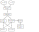
\includegraphics[width=\textwidth]{figures/functional-view}
\end{figure}

\subsection{Functional elements}
\label{sec:functional-elements}
These are the functional elements as presented in figure \ref{fig:funcView}.
They are grouped into 3 overall categories. The webserver part handles trafic
from users and admins, the Application process all interactions with the system,
and the database ensures persistence.

\textbf{WEBSERVER}

\begin{center}
  \begin{tabular}[h!]{| >{\columncolor{gray}}p{0.28\textwidth} | p{0.65\textwidth} |}
    \hline
    Element name & Cache\\
    \hline
    Responsibilities &
    \begin{itemize}
    \item Front layer to cache requests
    \item To increase performance of static parts
    \item Returns answers as a HTML-page
    \end{itemize}\\
    \hline
    Interfaces -- required & See figure \ref{fig:funcView}\\
    \hline
    Interfaces -- provided & See figure \ref{fig:funcView}\\
    \hline
  \end{tabular}
\end{center}

\begin{center}
  \begin{tabular}[h!]{| >{\columncolor{gray}}p{0.28\textwidth} | p{0.65\textwidth} |}
    \hline
    Element name & Request Handler\\
    \hline
    Responsibilities &
    \begin{itemize}
      \item Forwards user requests to Application layer
      \item Returns the HTML for a requested page.
    \end{itemize}\\
    \hline
    Interfaces -- required & See figure \ref{fig:funcView}\\
    \hline
    Interfaces -- provided & See figure \ref{fig:funcView}\\
   \hline
  \end{tabular}
\end{center}

\begin{center}
  \begin{tabular}[h!]{| >{\columncolor{gray}}p{0.28\textwidth} | p{0.65\textwidth} |}
    \hline
    Element name & Ajax\\
    \hline
    Responsibilities &
    \begin{itemize}
    \item Handles dynamic calls from webapplication.
    \item Returns XML for javascript on client.
    \end{itemize}\\
    \hline
    Interfaces -- required & See figure \ref{fig:funcView}\\
    \hline
    Interfaces -- provided & See figure \ref{fig:funcView}\\
    \hline
  \end{tabular}
\end{center}

\begin{center}
  \begin{tabular}[h!]{| >{\columncolor{gray}}p{0.28\textwidth} | p{0.65\textwidth} |}
    \hline
    Element name & Action Control\\
    \hline
    Responsibilities &
    \begin{itemize}
      \item Directs user requests
    \end{itemize}\\
    \hline
    Interfaces -- required & See figure \ref{fig:funcView}\\
    \hline
    Interfaces -- provided & See figure \ref{fig:funcView}\\
   \hline
  \end{tabular}
\end{center}

\begin{center}
  \begin{tabular}[h!]{| >{\columncolor{gray}}p{0.28\textwidth} | p{0.65\textwidth} |}
    \hline
    Element name & Query handler\\
    \hline
    Responsibilities &
    \begin{itemize}
      \item Translate requests to queries for
        \begin{itemize}
          \item Adding item
          \item Removing item
          \item Find item
          \item Queuing to item
        \end{itemize}
    \end{itemize}\\
    \hline
    Interfaces -- required & See figure \ref{fig:funcView}\\
    \hline
    Interfaces -- provided & See figure \ref{fig:funcView}\\
   \hline
  \end{tabular}
\end{center}

\begin{center}
  \begin{tabular}[h!]{| >{\columncolor{gray}}p{0.28\textwidth} | p{0.65\textwidth} |}
    \hline
    Element name & Item Store\\
    \hline
    Responsibilities &
    \begin{itemize}
      \item Interface for the storing and handling of items.
    \end{itemize}\\
    \hline
    Interfaces -- required & See figure \ref{fig:funcView}\\
    \hline
    Interfaces -- provided & See figure \ref{fig:funcView}\\
   \hline
  \end{tabular}
\end{center}

\begin{center}
  \begin{tabular}[h!]{| >{\columncolor{gray}}p{0.28\textwidth} | p{0.65\textwidth} |}
    \hline
    Element name & Transaction Handler\\
    \hline
    Responsibilities &
    \begin{itemize}
      \item Handles transactions for renting out items; \seller to \buyer
      \item Handles transactions for returning items; \buyer to \seller
      \item Redirects billing to third party billing service
      \item Asserts items exists
    \end{itemize}\\
    \hline
    Interfaces -- required & See figure \ref{fig:funcView}\\
    \hline
    Interfaces -- provided & See figure \ref{fig:funcView}\\
   \hline
  \end{tabular}
\end{center}

\begin{center}
  \begin{tabular}[h!]{| >{\columncolor{gray}}p{0.28\textwidth} | p{0.65\textwidth} |}
    \hline
    Element name & Event Log\\
    \hline
    Responsibilities &
    \begin{itemize}
      \item Logs transactions between users (renting of an item, returning of an item)
    \end{itemize}\\
    \hline
    Interfaces -- required & See figure \ref{fig:funcView}\\
    \hline
    Interfaces -- provided & See figure \ref{fig:funcView}\\
   \hline
  \end{tabular}
\end{center}

\begin{center}
  \begin{tabular}[h!]{| >{\columncolor{gray}}p{0.28\textwidth} | p{0.65\textwidth} |}
    \hline
    Element name & Payment proxy\\
    \hline
    Responsibilities &
    \begin{itemize}
    \item Internal interface between application and Payment Service
    \end{itemize}\\
    \hline
    Interfaces -- required & See figure \ref{fig:funcView}\\
    \hline
    Interfaces -- provided & See figure \ref{fig:funcView}\\
    \hline
  \end{tabular}
\end{center}

\begin{center}
  \begin{tabular}[h!]{| >{\columncolor{gray}}p{0.28\textwidth} | p{0.65\textwidth} |}
    \hline
    Element name & Admin\\
    \hline
    Responsibilities &
    \begin{itemize}
    \item Perform inspection of Item store and Event log.
    \end{itemize}\\
    \hline
    Interfaces -- required & See figure \ref{fig:funcView}\\
    \hline
    Interfaces -- provided & See figure \ref{fig:funcView}\\
    \hline
  \end{tabular}
\end{center}
\subsection{Functional scenarios}
\label{sec:functional-scenarios-1}
The two former functional scenarios are here presented in sequence diagrams.

\textbf{R1} - A user creating an item in the system, is presented in figure
\ref{fig:r1-sequence}

\textbf{R2} - The user finds and rents an item, is presented in figure
\ref{fig:r2-sequence}

\begin{figure}[ht]
    \centering
    \caption{The function scenario R1}
    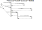
\includegraphics[width=0.8\textwidth]{figures/r1-sequence}
    \label{fig:r1-sequence}
\end{figure}

\begin{figure}[ht]
    \centering
    \caption{The function scenario R2}
    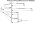
\includegraphics[width=0.8\textwidth]{figures/r2-sequence}
    \label{fig:r2-sequence}
\end{figure}



\subsection{System-wide processing}
\label{sec:syst-wide-proc}
Multiple events, like errors in message delivery (due to for example congestion on the network), can have effect on the whole system.
The system is build around Remote Procedure Calls (RPCs), implemented as messages, send over network via HTTP/HTTPS to different components (possible on different machines) handling different sides of data processing. Thus it is important to use selected schemes to handle for example atomicity, consistency, durability, etc. across all components in a consistent way -- the chain is only as strong as its weakest link.

We shall therefore use the ACID-methodology between clients and components:
\begin{itemize}
    \item \textbf{A}tomicity: all RPCs are atomic.
    \item \textbf{C}onsistency: all RPC are consistent (changes the component from one state to another).
    \item \textbf{I}solation: all RPCs have before-or-after atomicity.
    \item \textbf{D}urability: logging of RPCs ensures that the results of a done (commited) RPC is persistent.
\end{itemize}
such that the system is atomic, consistent, durable (at least with respect to persistent data).

We shall implement ACID using for example BASE (in the following, component refers to instance of thereof, not the abstract notion of component. Thus by a fail-stop of a component is meant the fail-stop of an instance of this component):
\begin{itemize}
    \item \textbf{B}asically-\textbf{A}vailable: Only failed components (read instances thereof) become unavailable, not any other components (especially not the whole system).
    \item \textbf{S}oft-state: Components can fail (fail-stop) without affecting availability of other components, but components may be out-of-date, e.g. an execution of a step, like registering an item, might not have returned and/or updated an item correctly before a crash of either one.
    \item \textbf{E}ventually consistent: Asynchronous calls between components ensures that an update step in the data flow is eventually executed, and that the component making the update is eventually consistent. For example an added item might not be visible to all other users as soon as the user admitting the item gets a notification of success -- but it will eventually be visible to all others.
\end{itemize}
When talking about asynchronous calls, this is only meant to be implemented internally -- users should not use asynchronous calls, as users needs responses of success or failure shortly after making an data updating/changing request, like removing or adding an item. But note that this does not mean that a successful request of adding an item can be seen by all other users.

To enable ACID, we shall also use a log-everything-scheme, meaning that every process is logged at each component. Thus errors can always be detected and or handled, if not at runtime, then later when running through the logs. Of course this needs special attention to make logs isolated from logs of other processes (e.g. so that we with certainty can say which process did a step first).

%TODO; maybe add an example

\section{Information view}
\label{cha:information-view}
%TODO?


\subsection{Data structure}
\label{sec:data-structure}
%TODO
The static data/information structure of ORS is shown in figure \ref{fig:data_struct}. All data is created and held by ORS itself. The figure shows the class structure (with for example Query and Event), but it also illustrates the attributes and primary keys (underlined attributes) used in the database system holding the data (note that a query is not stored and thus contains no primary key).

\begin{figure}[h!]
  \centering
  \caption{The data structure}
  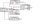
\includegraphics[width=0.8\textwidth]{figures/data_structure}
  \label{fig:data_struct}
\end{figure}


\subsection{Data flow}
\label{sec:data-flow}
The data flow follows from the functional views, but an elaborated version is found in figure \ref{fig:data_flow}. Note that the static data structures in figure \ref{fig:data_struct} is contained in \texttt{Event} and \texttt{Query}, as described in figure figure \ref{fig:data_struct}.

\begin{figure}[h!]
  \centering
  \caption{The data flow}
  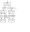
\includegraphics[width=0.8\textwidth]{figures/data_flow}
  \label{fig:data_flow}
\end{figure}

\subsection{Data ownership}
\label{sec:data-ownership}
All data used is created and owned by ORS. No external persistent data input exists (we have communication with some social medias and a billing system, but data transfered between them and the ORS system is not specifically owned by anyone nor stored in ORS).


\subsection{Information lifecycles}
\label{sec:inform-lifecycl}
%TODO
The information lifecycle of the user data is illustrated in figure \ref{fig:info_lifecyc0}. Other data follows the same structure.

\begin{figure}[h!]
  \centering
  \caption{Information life cycle of \texttt{User} information}
  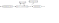
\includegraphics[width=0.8\textwidth]{figures/information_lifecycle0}
  \label{fig:info_lifecyc0}
\end{figure}


\subsection{Timeliness and latency}
\label{sec:timeliness-latency}
See section \ref{sec:syst-wide-proc} for more information on how latency and concurrency will be handled by the system.


\subsection{Archive and retention}
\label{sec:archive-retention}
User data should be hold by ORS as long as a user is active plus a couple of years after a user unsubscribes from the system. Audit of the firm needs information of transactions and user information within a the last couple of years, but after that it should not be needed and user data can then be deleted.

\newpage
\section{Concurrency view}
\label{sec:concurrency-view}


\subsection{Concurrency model}
\label{sec:concurrency-model}

\begin{figure}[h!]
    \centering
    \caption{The concurrency model}
    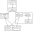
\includegraphics[width=0.8\textwidth]{figures/concurrency-model}
    \label{fig:concurrency-model}
\end{figure}

From figure\ref{fig:concurrency-model} it can be seen that the application consists of
three categrories of components, the webserver, the application and the database.
The webserver is the entry point for the application to relive this bottleneck
the application will be designed with a heavy degree of parallelism in mind.


Figure \ref{fig:} shows the concurrency model of our system.
The entry point being the webserver uses the Request Forwarder to distribute
requests over multiple workers. There are two primary worker groups, the Query
handlers and the Transaction handlers. These processes will all run virtualized on servers
created depending on the loadfactor of the system. This ensures that the request
handling, atleast, wont be the bottleneck of the system as it can scale
horizontally. The item store and event log runs on their own cloud servers with
associated databases. Depending on the exact database technology this might also
allow some degree of horizontal scaling.


\subsection{State model}
\label{sec:state-model}

\begin{figure}[h!]
  \centering
  \caption{The state model}
  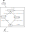
\includegraphics[width=0.8\textwidth]{figures/state-model}
  \label{fig:state-model}
\end{figure}

In figure\ref{fig:state-model} we see the state diagram for one conceptual
worker. Multiple request handlers can be spawned for both Querys and
Transactions as needed so we only look at the state for one such.
\section{Deployment view}
\label{sec:deployment-view}


\subsection{Runtime platform model}
\label{sec:runt-platf-model}

We will rely on Amazon's cloud services AWS for the infrastructure.
Most notably we will use EC2 virtual servers to run Application handlers, both
Query handlers, and Transaction handlers. For datastorage including the Item
store and the Event log we will use Amazon's DynamoDB instances and for static
content on the page we will use their S3 instances.

Amazon makes it easy to add further instances or scale up to better hardware,
this means we are not bound to a specific set of hardware requirements, instead
we can scale as currently needed.

Similarly it is possible to scale the size and throughput of our database
instance to suit our need.

\begin{figure}[h!]
  \centering
  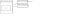
\includegraphics[width=0.9\textwidth]{figures/runtime-platform-model}
  \label{fig:runtime-platform-model}
  \caption{The runtime platform model}
\end{figure}


\subsection{Software dependencies}
\label{sec:softw-depend}
Our software requirements are fairly simple.
As we rely on Java we have very low requirements for operating systems which
fits our model of simple virtual machines well.
We will use AWS Elastic beanstalk as our way for deployment.

\begin{table}[h!]
  \centering
  \begin{tabular}[h]{l|l|l}
    Software & \textit{Library}  & Version \\
    \hline
    Java & & 8 \\
    & AWS SDK for Java & 1.8+ \\
    AWS Elastic Beanstalk & & \\
  \end{tabular}
  \caption{Software dependencies}
  \label{tab:software-dependencies}
\end{table}
\subsection{Network model}
\label{sec:network-model}

The network is handled by Amazon, we will simply have to track which services
are running where. Communication is done via HTTP REST requests so no special
network setup is needed.

\section{Development view}
\label{sec:development-view}
This section describes the environment the system is to be developed in. To
allow for the rapid changes in technologies, the environment description goes
into detail where possible, and leaves the choice open when necessary.

\subsection{Module structure}
\label{sec:module-structure}
The module structure is shown in figure \ref{fig:dev_module_structure}, where
the different modules has been categorized into layers.

\begin{figure}[ht]
    \centering
    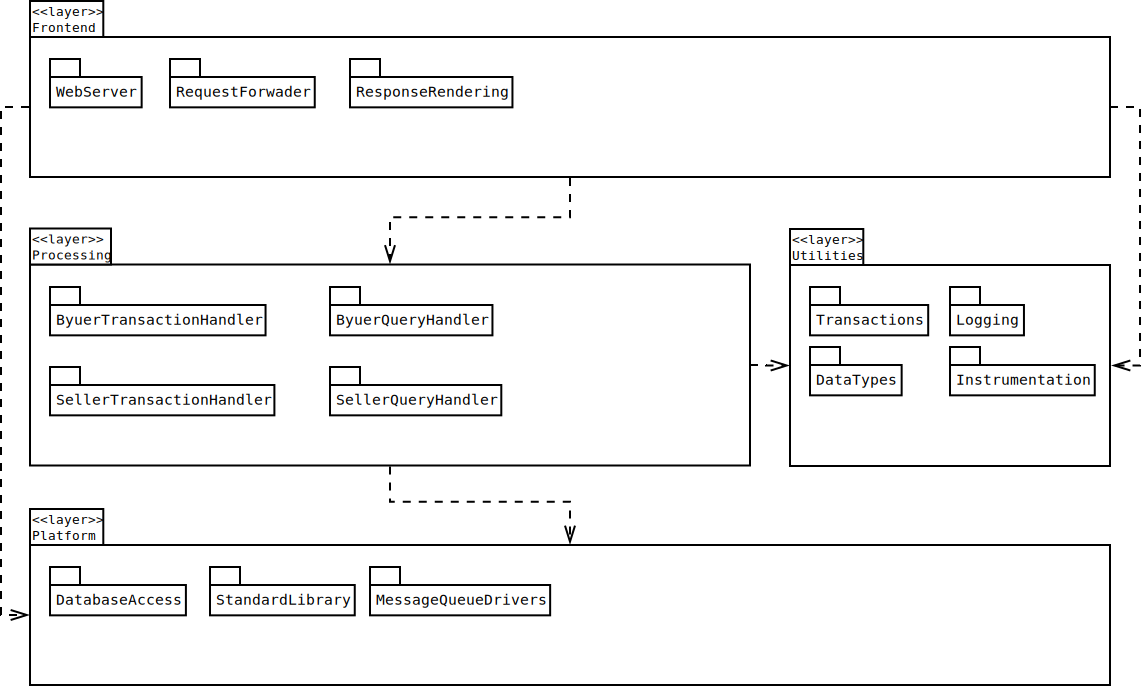
\includegraphics[width=0.9\textwidth]{figures/dev_module_structure}
    \label{fig:dev_module_structure}
    \caption{The modules and components decomposed into layers}
\end{figure}

\subsection{Common design}
\label{sec:common-design}
This section outlines common design goals for services and internal components.

\begin{itemize}
    \item All code components should utilize Dependency Injection for their
        internal dependencies. This shall be accomplished with the appropriate
        DI-container for the chosen environment.
    \item Logging in each component shall adhere to a standard message format.
        Furthermore to allow for interoperability between different systems, a
        common syslog or SNMP interface is desired. This aspect relates closely
        to the DI aspect and as such defines a strong reliance on modular code,
        that can be instrumented easily.
    \item Each component shall be run as a service, defining an interface
        either with an appropriate protocol or as a HTTP-service.
    \item Authentication shall be done between services. Services defining an
        HTTP interface shall use basic-auth, other protocols must define the
        necessary security primitives.
\end{itemize}

\subsection{Standards for design, code, and test}
\label{sec:stand-design-code}
In the following we briefly define the standards for developing the system. The
backbone of the development process is agile development, and as such the
standards define what needs to be done within one iteration and what processes
surround the development iterations, this relates closely to the operational
view(See section \ref{sec:operational-view}).

\begin{itemize}
    \item Components shall focus on one single task and only provide
        functionality within that scope. The interface for a component shall
        follow common guidelines for good interface design, and further adhere
        to the wish of DI.
    \item Building is done via the preferred or dictated build system for the
        chosen technical environment. If the environment doesn't specify one
        Apache Maven could be desirable.
    \item All modules/components must be contained within them self, and
        therefore unit tests are done separately for each unit of code. All
        modules must be registered with the central continuous integration
        system.
    \item Integration tests are kept within the main project, and are mainly
        targeted at nightly builds or builds intended for deployment.
    \item Configuration and source code shall be kept in separate version
        control repositories. The Git versioning system is chosen as the
        primary VC.
    \item The licence of external dependencies shall be as liberal as possible,
        but the guiding principle shall be quality of the external module.
\end{itemize}


\subsection{Codeline organization}
\label{sec:codel-organ}
The modules are expected to be self-contained and as such no common structure
is required. It is desired that each component gathers a group of modules,
which are contained in their own repository and included with the package
management system of choice within the chosen technical solution.

The main project is then reduced to glueing together the modules by starting
them and inserting instrumentation configuration where necessary.

\section{Operational view}
\label{sec:operational-view}
This section shows how the operational environment of the system is to be created and maintained. The components of this view are described in section \ref{sec:deployment-view}. In figure \ref{fig:logic_comp} we see the components to be installed and operated.

\begin{figure}[h!]
  \centering
  \caption{Overview of logical components}
  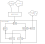
\includegraphics[width=0.8\textwidth]{figures/deployment_view}
  \label{fig:logic_comp}
\end{figure}


\subsection{Installation and migration}
\label{sec:inst-migr}
The following steps are required to install the ORS platform in reference of figure \ref{fig:logic_comp}.

Specifically for this installation guide, it is expected to be runned on Amazon cloud, utilizing AWS (Amazon Web Services) DynamoDB, AWS Beanstalk and AWS S3 (Simple Storage Service). Thus all components are logically divided (each to its own instance) and easily scaled up.

Note that this installation does not handle the configuration of the billing service.
\begin{enumerate}
    \item \label{enum:inst-migr_buy} Buy Amazon cloud services, DynamoDB,
    Beanstalk and S3. All following components is to be installed on these. Buy domain name and SSL certificates.
    \item \label{enum:inst-migr_wb} Install and configure the webserver (static files) (The configuration is currently setup via a text-based config-files, read at runtime) according to domains and certificates as of \ref{enum:inst-migr_buy}.
    \item \label{enum:inst-migr_db} Install and configure the database systems DynamoDB and Redis, handling \texttt{Item Store} and \texttt{Event log} respectively.
    \item \label{enum:inst-migr_bs} Get access to billing service and configure it to point to \ref{enum:inst-migr_buy}.
    \item Download and install Java 8.
    \item Install the backend, the Application layer, of ORS and configure it to point to location of \ref{enum:inst-migr_wb} and \ref{enum:inst-migr_db} (The configuration is currently setup via a text-based config-files, read at runtime). Note that the configuration of the payment proxy depends on \ref{enum:inst-migr_bs}. Internally of the Application layer, the cloud service provides and delegates addresses of instances.
    \item Test the installation by either manually accessing and using site or by automatic test cases (currently not developed).
\end{enumerate}

\subsection{Operational configuration management}
\label{sec:oper-conf-manag}
The system relies on the AmazonWebServices(AWS) to provide all underlying
infrastructure, this frees us from configuring operating systems and the actual
running software, except of course for the things developed.

The following configuration groups has been identified:

\begin{description}
    \item[AWS] The S3 storage and Route53 needs configuration, to host
        the static files for the website.
        Amazon Beanstalk,needs configuration for the parameters:
        scalability, performance and component specifics.
        Dynamo DB needs to be configured for the scalability parameters of
        the application components(Tuning the CAP).
    \item[Redis] requires us to maintain the operating system and the complete
        stack surrounding the Redis cluster.
\end{description}

It is identified that the Webserver and Application components share
configuration values for the endpoint-address configuration - within the AWS
configuration group.

This constitutes the component needing configuration. A somewhat larger
overhead is carried, due to the use of AWS, but the costs reduced by not
managing servers and OS is paramount.


\subsection{System administration}
\label{sec:syst-admin}
The main part of the system is deployed on AWS which as a platform provides
logging facilities and monitoring. It is planned to use these as much as
possible.

The Redis service is going to run on an EC2 instance, where we will utilise the
AWS SDK to report performance metrics and monitor the health of the services.

It is believed that the main way of system failure notification will be by SMS
and email, depending on severity.


\subsection{Provision of support}
\label{sec:provision-support}
Users are the only stakeholders that will recieve support through ORS. This support will be handled by administrators of the site as first level supporters and ORS developers at second level.

Administrators will also handle payment support, and might direct it to the chosen billing service provider.

Support is provided through an email going to the administrators, who can delegate cases to second level if necessary.
